%% Преамбула TeX-файла

% 1. Стиль и язык
\documentclass[utf8x, 12pt]{G7-32} % Стиль (по умолчанию будет 14pt)

% Остальные стандартные настройки убраны в preamble.inc.tex.
\sloppy

% Настройки стиля ГОСТ 7-32
% Для начала определяем, хотим мы или нет, чтобы рисунки и таблицы нумеровались в пределах раздела, или нам нужна сквозная нумерация.
\EqInChapter % формулы будут нумероваться в пределах раздела
\TableInChapter % таблицы будут нумероваться в пределах раздела
\PicInChapter % рисунки будут нумероваться в пределах раздела
\usepackage{slashbox}

% Добавляем гипертекстовое оглавление в PDF
\usepackage[
bookmarks=true, colorlinks=true, unicode=true,
urlcolor=black,linkcolor=black, anchorcolor=black,
citecolor=black, menucolor=black, filecolor=black,
]{hyperref}

% Изменение начертания шрифта --- после чего выглядит таймсоподобно.
% apt-get install scalable-cyrfonts-tex

\IfFileExists{cyrtimes.sty}
    {
        \usepackage{cyrtimespatched}
    }
    {
        % А если Times нету, то будет CM...
    }

\usepackage{graphicx}   % Пакет для включения рисунков

% С такими оно полями оно работает по-умолчанию:
% \RequirePackage[left=20mm,right=10mm,top=20mm,bottom=20mm,headsep=0pt]{geometry}

\geometry{right=20mm}
\geometry{left=30mm}


% Пакет Tikz
\usepackage{tikz}
\usetikzlibrary{arrows,positioning,shadows}
\usepackage{pgfplots}

% Произвольная нумерация списков.
\usepackage{enumerate}

% ячейки в несколько строчек
\usepackage{multirow}

% itemize внутри tabular
\usepackage{paralist,array}

% Центрирование подписей к плавающим окружениям
\usepackage[justification=centering]{caption}

% My

\usepackage[export]{adjustbox}
\usepackage{float}


% Настройки листингов.
\ifPDFTeX
% Листинги

\usepackage{listings}
\usepackage{wrapfig}
% Значения по умолчанию
\lstset{
  basicstyle= \footnotesize,
  breakatwhitespace=true,% разрыв строк только на whitespacce
  breaklines=true,       % переносить длинные строки
%   captionpos=b,          % подписи снизу -- вроде не надо
  inputencoding=koi8-r,
  numbers=left,          % нумерация слева
  numberstyle=\footnotesize,
  showspaces=false,      % показывать пробелы подчеркиваниями -- идиотизм 70-х годов
  showstringspaces=false,
  showtabs=false,        % и табы тоже
  stepnumber=1,
  tabsize=4,              % кому нужны табы по 8 символов?
  frame=single,
  escapeinside={(*}{*)}, %выделение
  literate={а}{{\selectfont\char224}}1
  {б}{{\selectfont\char225}}1
  {в}{{\selectfont\char226}}1
  {г}{{\selectfont\char227}}1
  {д}{{\selectfont\char228}}1
  {е}{{\selectfont\char229}}1
  {ё}{{\"e}}1
  {ж}{{\selectfont\char230}}1
  {з}{{\selectfont\char231}}1
  {и}{{\selectfont\char232}}1
  {й}{{\selectfont\char233}}1
  {к}{{\selectfont\char234}}1
  {л}{{\selectfont\char235}}1
  {м}{{\selectfont\char236}}1
  {н}{{\selectfont\char237}}1
  {о}{{\selectfont\char238}}1
  {п}{{\selectfont\char239}}1
  {р}{{\selectfont\char240}}1
  {с}{{\selectfont\char241}}1
  {т}{{\selectfont\char242}}1
  {у}{{\selectfont\char243}}1
  {ф}{{\selectfont\char244}}1
  {х}{{\selectfont\char245}}1
  {ц}{{\selectfont\char246}}1
  {ч}{{\selectfont\char247}}1
  {ш}{{\selectfont\char248}}1
  {щ}{{\selectfont\char249}}1
  {ъ}{{\selectfont\char250}}1
  {ы}{{\selectfont\char251}}1
  {ь}{{\selectfont\char252}}1
  {э}{{\selectfont\char253}}1
  {ю}{{\selectfont\char254}}1
  {я}{{\selectfont\char255}}1
  {А}{{\selectfont\char192}}1
  {Б}{{\selectfont\char193}}1
  {В}{{\selectfont\char194}}1
  {Г}{{\selectfont\char195}}1
  {Д}{{\selectfont\char196}}1
  {Е}{{\selectfont\char197}}1
  {Ё}{{\"E}}1
  {Ж}{{\selectfont\char198}}1
  {З}{{\selectfont\char199}}1
  {И}{{\selectfont\char200}}1
  {Й}{{\selectfont\char201}}1
  {К}{{\selectfont\char202}}1
  {Л}{{\selectfont\char203}}1
  {М}{{\selectfont\char204}}1
  {Н}{{\selectfont\char205}}1
  {О}{{\selectfont\char206}}1
  {П}{{\selectfont\char207}}1
  {Р}{{\selectfont\char208}}1
  {С}{{\selectfont\char209}}1
  {Т}{{\selectfont\char210}}1
  {У}{{\selectfont\char211}}1
  {Ф}{{\selectfont\char212}}1
  {Х}{{\selectfont\char213}}1
  {Ц}{{\selectfont\char214}}1
  {Ч}{{\selectfont\char215}}1
  {Ш}{{\selectfont\char216}}1
  {Щ}{{\selectfont\char217}}1
  {Ъ}{{\selectfont\char218}}1
  {Ы}{{\selectfont\char219}}1
  {Ь}{{\selectfont\char220}}1
  {Э}{{\selectfont\char221}}1
  {Ю}{{\selectfont\char222}}1
  {Я}{{\selectfont\char223}}1
}

% Стиль для псевдокода: строчки обычно короткие, поэтому размер шрифта побольше
\lstdefinestyle{pseudocode}{
  basicstyle=\small,
  keywordstyle=\color{black}\bfseries\underbar,
  language=Pseudocode,
  numberstyle=\footnotesize,
  commentstyle=\footnotesize\it
}

% Стиль для обычного кода: маленький шрифт
\lstdefinestyle{realcode}{
  basicstyle=\scriptsize,
  numberstyle=\footnotesize
}

% Стиль для коротких кусков обычного кода: средний шрифт
\lstdefinestyle{simplecode}{
  basicstyle=\footnotesize,
  numberstyle=\footnotesize
}

% Стиль для BNF
\lstdefinestyle{grammar}{
  basicstyle=\footnotesize,
  numberstyle=\footnotesize,
  stringstyle=\bfseries\ttfamily,
  language=BNF
}

% Определим свой язык для написания псевдокодов на основе Python
\lstdefinelanguage[]{Pseudocode}[]{Python}{
  morekeywords={each,empty,wait,do},% ключевые слова добавлять сюда
  morecomment=[s]{\{}{\}},% комменты {а-ля Pascal} смотрятся нагляднее
  literate=% а сюда добавлять операторы, которые хотите отображать как мат. символы
    {->}{\ensuremath{$\rightarrow$}~}2%
    {<-}{\ensuremath{$\leftarrow$}~}2%
    {:=}{\ensuremath{$\leftarrow$}~}2%
    {<--}{\ensuremath{$\Longleftarrow$}~}2%
}[keywords,comments]

% Свой язык для задания грамматик в BNF
\lstdefinelanguage[]{BNF}[]{}{
  morekeywords={},
  morecomment=[s]{@}{@},
  morestring=[b]",%
  literate=%
    {->}{\ensuremath{$\rightarrow$}~}2%
    {*}{\ensuremath{$^*$}~}2%
    {+}{\ensuremath{$^+$}~}2%
    {|}{\ensuremath{$|$}~}2%
}[keywords,comments,strings]

% Подписи к листингам на русском языке.
\renewcommand\lstlistingname{\cyr\CYRL\cyri\cyrs\cyrt\cyri\cyrn\cyrg}
\renewcommand\lstlistlistingname{\cyr\CYRL\cyri\cyrs\cyrt\cyri\cyrn\cyrg\cyri}

\else
\usepackage{local-minted}
\fi

% Полезные макросы листингов.
% Любимые команды
\newcommand{\Code}[1]{\textbf{#1}}


\begin{document}

\frontmatter % выключает нумерацию ВСЕГО; здесь начинаются ненумерованные главы: реферат, введение, глоссарий, сокращения и прочее.

% Команды \breakingbeforechapters и \nonbreakingbeforechapters
% управляют разрывом страницы перед главами.
% По-умолчанию страница разрывается.

% \nobreakingbeforechapters
% \breakingbeforechapters

% Также можно использовать \Referat, как в оригинале
%\begin{abstract}
%	Титульный лист. Эта страница нужна мне, чтобы не сбивалась нумерация страниц
%	\cite{Dh}
%	\cite{Bayer}
%	\cite{Habr1}
%	\cite{Noise_func}
%	\cite{Ulich}

%Это пример каркаса расчётно-пояснительной записки, желательный к использованию в РПЗ проекта по курсу РСОИ.

%Данный опус, как и более новые версии этого документа, можно взять по адресу (\url{https://github.com/rominf/latex-g7-32}).

%\end{abstract}
% НАЧАЛО ТИТУЛЬНОГО ЛИСТА
\begin{center}
	\bigbreak
	\textit{
		Государственное образовательное учреждение высшего профессионального образования}\\ 
	
	\textit{
		\noindent
		\begin{minipage}{0.2\textwidth}% adapt widths of minipages to your needs
			
\includegraphics[scale=0.5]{img/bmstu-logo.png}~
		\end{minipage}
		\hfill
		\begin{minipage}{0.7\textwidth}\centering
		    \bf  «Московский государственный технический университет\\ 
			\bf имени Н. Э. Баумана»\\
			\bf (МГТУ им. Н.Э. Баумана)\\
		\end{minipage}
		\bigbreak
	}
	
	\noindent\rule{\textwidth}{2pt}
	\bigbreak
	

	\noindent
	\begin{minipage}{0.15\textwidth}\raggedright
		ФАКУЛЬТЕТ\\
		КАФЕДРА
	\end{minipage}
	\hfill
	\begin{minipage}{0.8\textwidth}\centering
		«Информатика и системы управления»\\
		«Программное обеспечение ЭВМ и информационные технологии»
	\end{minipage}
	
	\vspace{\fill}
	\normalsize{\bf Р А С Ч Ё Т Н О - П О Я С Н И Т Е Л Ь Н А Я\space\space З А П И С К А}\\
	\normalsize{\bf к курсовой работе на тему:}\\
	\large{<<Программа для бесконтактного оптического измерения геометрических параметров объекта>>}\\\vspace{\fill}	
	\normalsize {
		\noindent
		\makebox[0pt][l]{Студент}%
		\makebox[\textwidth][c]{}%
		\makebox[0pt][r]{{$\underset{\text{(Подипсь, дата)}}{\underline{\hspace{6cm}}}$ \space Анисимов Н.С.}}
	}\\
	\bigbreak	
	\normalsize {
		\noindent
		\makebox[0pt][l]{Руководитель курсового проекта}%
		\makebox[\textwidth][c]{ ~~~~~~~~      }%
		\makebox[0pt][r]{{$\underset{\text{(Подпись, дата)}}{\underline{\hspace{6cm}}}$ \space\space\space\space\space\space Куров А.В.}}
	}
\end{center}
\vspace{\fill}
\begin{center} Москва 2017 \end{center}

\thispagestyle{empty} % 
% КОНЕЦ ТИТУЛЬНОГО ЛИСТА


%%% Local Variables: 
%%% mode: latex
%%% TeX-master: "rpz"
%%% End: 

\tableofcontents

\Introduction

Промышленные измерительные системы позволяют проводить бесконтактные измерения геометрических размеров и формы сырья, заготовок, деталей и готовой продукции в процессе производства непосредственно на конвейере или в производственной линии.

В настоящее время ставится задача разработки программного обеспечения, позволяющего обрабатывать графические изображения (фотографии или видео) и определять геометрические параметры объектов (исходных заготовок произвольной формы), находящихся на движущемся конвейере или непосредственно в зоне обработки, для выдачи корректирующего сигнала в общую систему адаптивного контроля и управления кузнечно-прессовым оборудованием.

Целью данной работы является измерение геометрических параметров цилиндра, изображенном на фотографии, а так же визуализации процесса движения цилиндра по конвейеру.

\mainmatter % это включает нумерацию глав и секций в документе ниже

\chapter{ Аналитический раздел }
Данный раздел посвящен анализу предметной области и задачи распознавания цилиндра и нахождения его геометрических размеров. Здесь также проводится обзор существующих методов и алгоритмов, позволяющих решить эту задачу.
Формально, алгоритм нахождения размеров состоит из нескольких шагов:
\begin{enumerate}
	\item Выделение границ цилиндра 
	\item Нахождение боковых граней цилиндра 
	\item На основе расстояния между найденными гранями и параметров камеры, вычислить размеры 
\end{enumerate}

Далее так же приводится анализ алгоритм трехмерного моделирования.

\section{ Анализ алгоритмов нахождения границ изображения }
Для решения данной задачи, было разработаны большое количество алгоритмов. Далее приведено описание наиболее популярных и используемых.
Также для ускорения работы алгоритмов, изображение желательно перевести в градации серого путем вычисления средневзвешенного количества красного, зеленого и синего цветов. в. Используется формула
\[Y = 0.3*R + 0.59*G + 0.11*B\]
эта величина также известна как свечение. Коэффициенты, используемые для расчета свечения, выбраны из соображений особенностей человеческого восприятия. Дело в том, что из базовых цветов, взятых в одинаковом количестве, человеческих глаз сперва выделяет зеленый, затем красный, а уже потом синий. Подразумевается, что когда зеленый и синий цвета излучаются монитором в одинаковом количестве, зеленый, тем не менее, выглядит ярче. Поэтому преобразование в градации серого цвета путем вычисления среднего арифметического цветовых компонент не отражает воспринимаемую человеком яркость оригинала. Для этого используется средневзвешенная величина.


\subsection{Оператор Собеля}
\label {sobel}
Оператор Собеля – дискретный дифференциальный оператор, вычисляющий приближенные значения производных разного порядка для функции яркости пикселей [1]. Наиболее распространенным примером практического использования является определение границ (ребер) объектов на изображении, т.е. точек резкого изменения яркости.

Данный оператор основан на свертке изображения с целочисленными фильтрами. В простейшем случае оператор построен на вычислении сверток исходного изображения с ядрами \(G_x\) и \(G_y\) , обеспечивающими вычисление первых производных по направлениям:


\begin{gather}
G_{x}=
\begin{bmatrix} 
-1 & 0 & 1 \\ 
-2 & 0 & 2 \\ 
-1 & 0 & 1
\end{bmatrix},
G_{y}=
\begin{bmatrix}
-1 & -2 & -1 \\ 
0 & 0 & 0 \\ 
1 & 2 & 1
\end{bmatrix}
\end{gather}

Данный оператор используется для приближенного вычисления градиента функции интенсивности пикселей. Применение оператора \(G_{x}\) позволяет определить приближенное значение первой частной производной изменения интенсивности в горизонтальном направлении, \(G_{y}\) – в вертикальном. На основании данной информации можно вычислить магнитуду градиента для пикселя с координатами (i,j) согласно формуле \(\mid G^{ij} \mid = \sqrt{(G_{x}^{ij})^2 + (G_{y}^{ij})^2}\). Также используя полученные данные, можно определить направление градиента как \(\theta^{ij} = arctan\left( \frac{G_{y}}{G_{x}}\right)\).

\subsection{Оператор Приютта}
Оператор Прюитта похож на оператор Собеля, но используются другие ядра:

\begin{gather}
G_{x}=
\begin{bmatrix} 
-1 & 0 & 1 \\ 
-1 & 0 & 1 \\ 
-1 & 0 & 1
\end{bmatrix},
G_{y}=
\begin{bmatrix}
-1 & -1 & -1 \\ 
0 & 0 & 0 \\ 
1 & 1 & 1
\end{bmatrix}
\end{gather}

\subsection{Оператор Робертса}
Оператор Робертса — один из ранних алгоритмов выделения границ, который вычисляет сумму квадратов разниц между диагонально смежными пикселами. Это может быть выполнено сверткой изображения с двумя ядрами:

\begin{gather}
G_{1}=
\begin{bmatrix} 
	1 & 0 \\ 
	0 & -1 \\ 
\end{bmatrix},
G_{2}=
\begin{bmatrix} 
	0 & 1 \\ 
	-1 & 0 \\ 
\end{bmatrix},
\end{gather}.

\subsection{Оператор Кэнни}
Данный алгоритм был разработан Джоном Кэнии в 1986 году. Его целью было разработать алгоритм алгоритм, который был бы оптимален по следующим критериям:
\begin{enumerate}
	\item Определение: вероятность определения точек реальных ребер должна быть максимальна, в то время как вероятность нахождения точек ложных ребер должна быть минимальна.
	\item Локализация: определенные ребра должны быть максимально близко к реальным ребрам.
	\item Количество ответов: одно реальное ребро, должно давать не более одного распознанного ребра.
\end{enumerate}
Алгоритм состоит из следующих пяти шагов.

\textbf{Сглаживание.} Неминуемо, что каждая фотография будет иметь некоторые шумы. Чтобы предотвратить ошибочное определение шумов как ребер, необходимо их удалить. Для этого к изображению применяется фильтр Гаусса. 
Ядро фильтра Гаусса с нормальным распределением \(\sigma = 1.4\) выглядит следующим образом:

\begin{gather} {B} ={\frac {1}{159}}{\begin{bmatrix}2&4&5&4&2\\4&9&12&9&4\\5&12&15&12&5\\4&9&12&9&4\\2&4&5&4&2\end{bmatrix}} \end{gather}

\textbf{Поиск градиентов.} 
Алгоритм Кэнни находит границы там, где интенсивность изображения меняется больше всего. Эти области находятся вычислением значений и направлений градиента. Градиент можно найти применением оператора Собеля, описанном в пункте \ref{sobel}.

\textbf{Подавление немаксимумов.} 
Целью данного шага является преобразование ``размытых'' границ на изображении градиентов в ``четкие''. Это может сделано сохранением всех локальных максимумов и подавлением всего остального. Алгоритм для каждого пикселя выглядит следующим образом:
\begin{itemize}
	\item Округление направления градиента \(\theta\) до ближайшего значения, кратного \(45^\circ\).
	\item Сравнение значения текущего пикселя, со значениями пекселей в положительном и отрицательном направлении градиента.
	\item Если значение текущего пикселя наибольшее, то сохраняем, иначе -- подавляем.
\end{itemize}

\textbf{Двойная пороговая фильтрация.} 
Пиксели, оставшиеся после предыдущего шага, вероятнее всего действительно будут ребрами, но некоторые из них могут быть получены из-за шумов или изменения цвета. Детектор границ Кэнни использует двойную пороговую фильтрацию. Пиксели, значения которых больше, чем верхняя граница, помечаются как ``сильные''. Пиксели, значения которых меньше, чем нижняя граница, подавляются, и пиксели, значения которых находятся между двумя границами помечаются как ``слабые''.

\textbf{Трассировка области неоднозначности.}
``Сильные'' пиксели, оставшиеся после предыдущего шага сразу добавляются в результирующие изображение. ``Слабые'' пиксели будут добавлены только в том случае, если они соприкасаются с ``сильными''.

\section{Анализ алгоритма нахождения прямых линий}
Наиболее распространенным алгоритмом поиска прямых является преобразование Хафа.
В простейшем случае преобразование Хафа является линейным преобразованием для обнаружения прямых. Прямая может быть задана уравнением \(y = mx + b\) и может быть вычислена по любой паре точек \((x, y)\) на изображении. Главная идея преобразования Хафа — учесть характеристики прямой не как уравнение, построенное по паре точек изображения, а в терминах её параметров, то есть \(m\) — коэффициента наклона и \(b\) — точки пересечения с осью ординат. Исходя из этого прямая, заданная уравнением \(y = mx + b\), может быть представлена в виде точки с координатами \((b, m)\) в пространстве параметров.

Однако прямые, параллельные оси ординат, имеют бесконечные значения для параметра \(m\). Поэтому удобней представить прямую с помощью других параметров, известных как \(r\) и \(\theta\). Параметр \(r\)  — это длина радиус-вектора ближайшей к началу координат точки на прямой (т.е. нормали к прямой, проведенной из начала координат), а \(\theta\) — это угол между этим вектором и осью абсцисс. При таком описании прямых не возникают бесконечные параметры.

Таким образом, уравнение прямой можно записать как:
\begin{gather}
y = \frac{-\cos{\theta}}{\sin{\theta}}x + \frac{r}{\sin {\theta}}
\end{gather}
или
\begin{gather}
r = x\cos{\theta} + y\sin{\theta}
\end{gather}

\section{Анализ алгоритмов удаление невидимых линий}
\subsection{Алгоритм Робертса}
Алгоритм Робертса представляет собой первое известное решение задачи об удалении невидимых линий. Это метод, работающий в объектном пространстве. В соответствии с алгоритмом, прежде всего удаляются из каждого тела те ребра или грани, которые перекрываются самим телом. Затем каждое из видимых ребер каждого тела сравнивается с каждым из оставшихся тел для определения того, какая его часть или части, если таковые есть, перекрываются этими телами.
 
Преимущества данного алгоритма в том, что математические методы, используемые в нем, просты, мощны и точны. Более поздние реализации алгоритма, например использующие предварительную сортировку вдоль оси z, демонстрируют почти линейную зависимость от числа объектов.

Минус этого алгоритма в том, что вычислительная трудоемкость алгоритма Робертса растет теоретически, как квадрат числа объектов. Реализация оптимизированных алгоритмов весьма сложна.

\subsection{Трассировка лучей}
В этом методе для каждого пикселя картинной плоскости определяется ближайшая к нему грань, для чего через этот пиксель выпускается луч, находятся все его пересечения с гранями и среди них выбирается ближайшая. 

К достоинствам данного алгоритма можно отнести возможность получения изображения гладких объектов без аппроксимации их примитивами (например, треугольниками). Вычислительная сложность метода линейно зависит от сложности сцены. Нетрудно реализовать наложение света и тени на объекты. Качество полученного изображения получается очень реалистичным, этот метод отлично подходит для создания фотореалистичных картин.

Серьёзным недостатком алгоритма трассирования является производительность. Для получения изображения необходимо создавать огромное число лучей, проходящих через сцену и отражаемых от объекта. Это приводит к существенному снижению скорости работы программы.

\subsection{Алгоритм, использующий z-буффер}
Алгоритм, использующий z-буфер это один из простейших алгоритмов удаления невидимых поверхностей. Впервые он был предложен Кэтмулом. Работает этот алгоритм в пространстве изображения. Идея z-буфера является простым обобщением идеи о буфере кадра. Буфер кадра используется для запоминания атрибутов (интенсивности) каждого пиксела в пространстве изображения, z-буфер - это отдельный буфер глубины, используемый для запоминания координаты z или глубины каждого видимого пиксела в пространстве изображения. В процессе работы глубина или значение z каждого нового пиксела, который нужно занести в буфер кадра, сравнивается с глубиной того пиксела, который уже занесен в z-буфер. Если это сравнение показывает, что новый пиксел расположен впереди пиксела, находящегося в буфере кадра, то новый пиксел заносится в этот буфер и, кроме того, производится корректировка z-буфера новым значением z. Если же сравнение дает противоположный результат, то никаких действий не производится. По сути, алгоритм является поиском по х и у наибольшего значения функции \(z(x,y)\).

Главное преимущество алгоритма – его простота. Кроме того, этот алгоритм решает задачу об удалении невидимых поверхностей и делает тривиальной визуализацию пересечений сложных поверхностей. Сцены могут быть любой сложности. Поскольку габариты пространства изображения фиксированы, оценка вычислительной трудоемкости алгоритма не более чем линейна. Поскольку элементы сцены или картинки можно заносить в буфер кадра или в z-буфер в произвольном порядке, их не нужно предварительно сортировать по приоритету глубины. Поэтому экономится вычислительное время, затрачиваемое на сортировку по глубине.

Основной недостаток алгоритма - большой объем требуемой памяти. Если сцена подвергается видовому преобразованию и отсекается до фиксированного диапазона значений координат z, то можно использовать z-буфер с фиксированной точностью. Информацию о глубине нужно обрабатывать с большей точностью, чем координатную информацию на плоскости \((x, y)\); обычно бывает достаточно 20-ти бит. Буфер кадра размером 512x512x24 бит в комбинации с z-буфером размером 512x512x20 бит требует почти 1.5 мегабайт памяти. Однако снижение цен на память делает экономически оправданным создание специализированных запоминающих устройств для z-буфера и связанной с ним аппаратуры.

\section{Анализ модели освещения по Фонгу}
Расчет освещения по Фонгу требует вычисления цветовой интенсивности трех компонент освещения: фоновой, рассеянной  и глянцевых бликов . Фоновая компонента — грубое приближение лучей света, рассеянных соседними объектами и затем достигших заданной точки; остальные две компоненты имитируют рассеивание и отражение прямого излучения.

Иллюстрация различных компонент, соединенных в модели Фонга
\begin{gather}
{\displaystyle I=K_{a}I_{a}+K_{d}({\vec {n}},{\vec {l}})+K_{s}({\vec {n}},{\vec {h}})^{p}}
\end{gather}

где

\({\displaystyle {\vec {n}}} \) — вектор нормали к поверхности в точке

\({\displaystyle {\vec {l}}} \)— направление проецирования (направление на источник света)

\({\displaystyle {\vec {h}}} \) — направление на наблюдателя

\({\displaystyle K_{a}}\) — коэффициент фонового освещения

\({\displaystyle K_{s}} \) — коэффициент зеркального освещения

\({\displaystyle K_{d}}\) — коэффициент диффузного освещения

\section{Выводы и выбор алгоритмов для поставленной задачи}
В качестве алгоритма выделения границ был использован на детектор границ Кэнни. Этот алгоритм дает наиболее точную границу, по сравнению со всеми выше описанными. Трансформация Хафа была использована для нахождения проекций цилиндрической поверхности.

Для удаления невидимых граней в трехмерной анимации был выбран алгоритм z-буффера. В силу простоты сцены, нет необходимости использовать эффективные алгоритмы, но в тоже время для сохранения плавности анимации нельзя использовать ресурсоемкие алгоритмы.

\chapter{Конструкторский раздел}
В данном разделе приводится описание общей структуры разрабатываемой системы, её основных модулей и структур данных. Подробно описываются методы и алгоритмы, выбранные для использования в системе.
\section{Структуры данных, используемых при нахождении размеров цилиндра}
Для нахождения геометрических размеров цилиндра использовались следующие структуры данных:

\begin{itemize}
	\item \texttt{Vector2.}
	Двухмерный вектор. Содержит в себе два атрибута, координаты \texttt{x} и \texttt{y}.
	
	\item \texttt{CylinderSize.}
	Размер цилиндра. Содержит в себе два атрибута, высоту \texttt{H} и радиус \texttt{R}.
	
	\item \texttt{Line.}
	Отрезок. Содержит в себе два атрибута, вектор \texttt{v1} и вектор v2.
	
	\item \texttt{Color.}
	Цвет. Содержит в себе три атрибута, соответствующие значения цветовых каналов \texttt{r, g, b}.
	
	\item \texttt{ImageBase.} 
	Базовый тип изображения, от него наследуются цветное изображение \texttt{ColorImage} и изображение в градациях серого \texttt{GrayscaleImage}.
	Содержит в себе массив значений пикселей изображения.
\end{itemize}
%
%\begin{figure}[H]
%	\centering
%	{
%		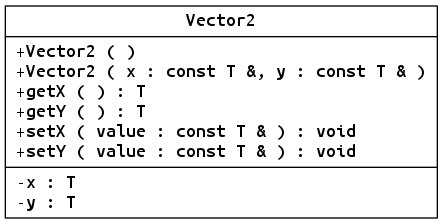
\includegraphics[scale=0.35,valign=t]{structs/Vector2.png}
%		\caption{}
%		\label{struct:types1}}
%\end{figure}
%\begin{figure}[H]
%	\centering
%	{
%		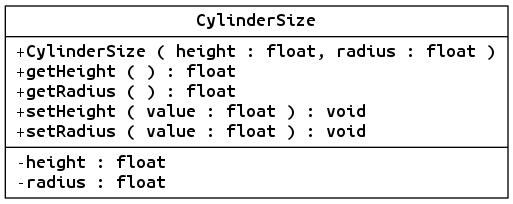
\includegraphics[scale=0.35,valign=t]{structs/CylinderSize.png}
%		\caption{Размеры цилиндра.}
%		\label{struct:types2}}
%\end{figure}
%\begin{figure}[H]
%	\centering
%	{
%		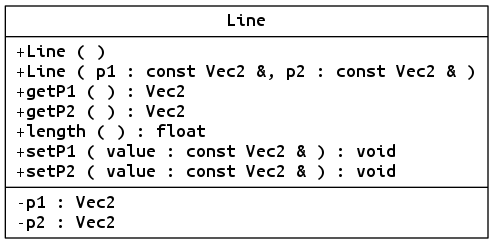
\includegraphics[scale=0.35,valign=t]{structs/Line.png}
%		\caption{Прямая.}
%		\label{struct:types3}}
%\end{figure}
%\begin{figure}[H]
%	\centering
%	{
%		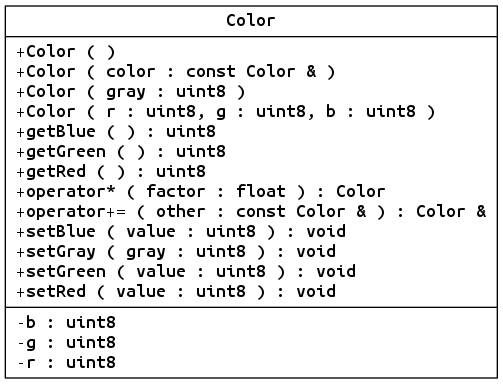
\includegraphics[scale=0.35,valign=t]{structs/Color.png}
%		\caption{Цвет.}
%		\label{struct:types4}}
%\end{figure}
%\begin{figure}[H]
%	\centering
%	{
%		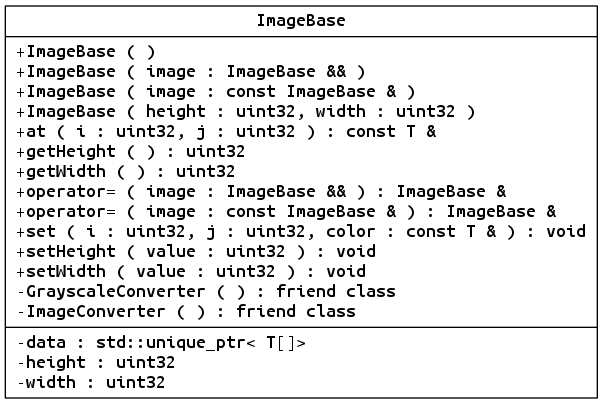
\includegraphics[scale=0.35,valign=t]{structs/ImageBase.png}
%		\caption{Базовый тип изображения, от него наследуются цветное изображение и изображение в градациях серого.}
%		\label{struct:types5}}
%\end{figure}

\section{Алгоритм нахождения размеров цилиндра}
Схема алгоритма нахождения размеров цилиндра представлена на рисунке \ref{fc:1}.
\begin{figure}[ht!]
	\centering{ 
		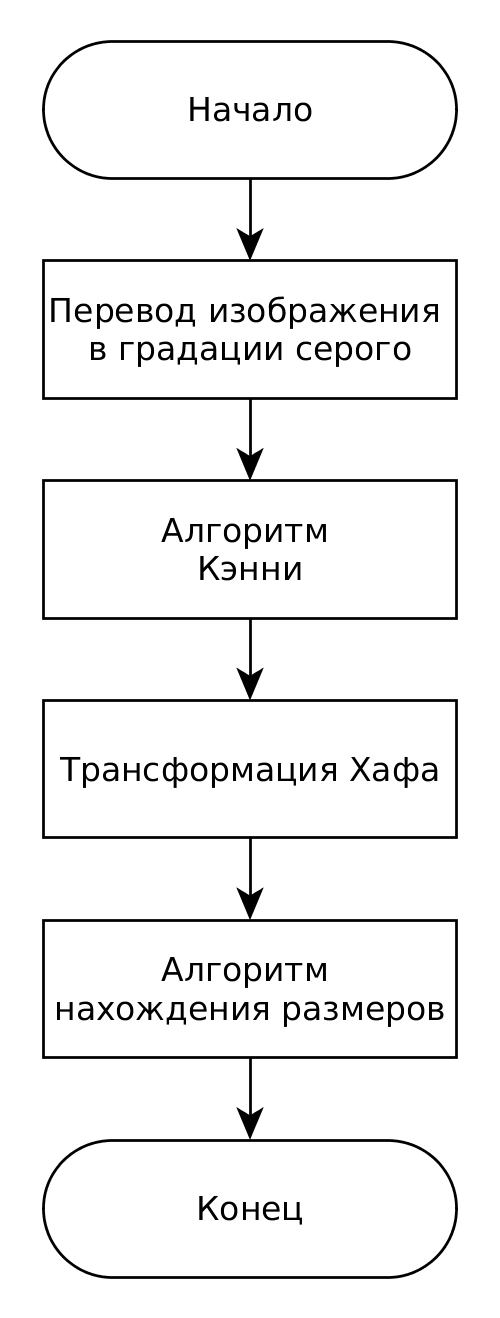
\includegraphics[width=0.32\textwidth]{img/fc1.png}
		\caption{Схема алгоритма нахождения размеров}
		\label{fc:1}}
\end{figure}




\section{Решение задачи определения геометрических размеров цилиндра}
При съемке цилиндра, с указанной позиции, диаметр цилиндра не виден полностью, а лишь его часть, как показано на рисунке \ref{an:vis}.

Зависимость размера видимой части цилиндра от высоты камеры \(CD = H\) и радиуса \(R\) можно вычислить согласно уравнениям (\eqref{eq:1}) - (\eqref{eq:2}).

\begin{gather}
\sin {\angle {ACO} } = \frac{AO}{CO} = \frac{R}{H-R} \label{eq:1} \\
\cos {\angle {ACO}} = \sqrt{1 - \sin ^2 {ACO}} = \sqrt {1 - (\frac {R}{H-R} )^ 2}\\ 
AE = R\cos {\angle {OAE}} = R\cos {\angle {ACO}} = R\sqrt {1 - (\frac {R}{H-R} )^ 2} \\
AB = 2AE = 2R\sqrt {1 - (\frac {R}{H-R} )^ 2} \label{eq:2}
\end{gather}

\begin{figure}[ht!]
	\centering{ 
		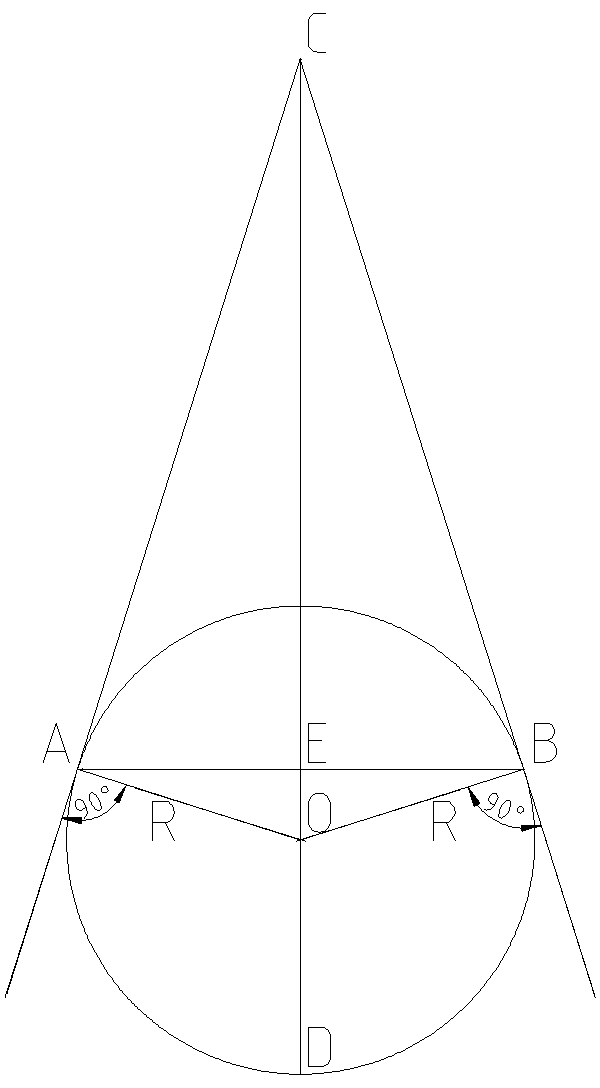
\includegraphics[width=0.3\textwidth]{img/analysis_1.png}
		\caption{Видимость цилиндра}
		\label{an:vis}}
\end{figure}

Длина \(AB\) будет соответствовать одному определенному значению радиуса \(R\) на промежутке \(I\), на котором длина \(AB\) возрастает. Верхнюю границу промежутка \(I\) можно найти из производной функции~\eqref{eq:1}.
Для случая, когда камера расположена на высоте \(H = 1\) метр, действителен следующий график:

\begin{figure}[ht!]
	\centering{ 
		\begin{tikzpicture}
		\begin{axis}[ 
		xmin=0,   xmax=1,
		ymin=0,   ymax=1,
		samples=401,
		xlabel=$R$,
		ylabel={$AB(R)$},
		] 
		\addplot [mark = none]{2*x*(1 - ( x/(1-x) )^ 2)^0.5 }; 
		\end{axis}
		\end{tikzpicture}
		\caption{Зависимость AB(R)}
		\label{an:vis1}
	}
\end{figure}

Из данной зависимости видно, что для корректной работы алгоритма, для данного случая, радиус цилиндра не должен превышать значение \(R=0.38197\) метра. В противном случае возникает неоднозначность.
Таким образом для промежутка \(I\) значение \(AB\) однозначно соответствует радиусу цилиндра и возможно однозначно определить высоту на которой находится \(AB\), и это значение можно использовать для вычисления масштабного коэффициента.

В вычислениях было сделано допущение, что лучи сходятся в одной точке. На самом же деле, лучи равномерно попадают на матрицу, которая имеет некоторые линейные размеры. Они были опушены, для упрощения вычислений и настройки программы.

\section{Структуры данных, используемых для трехмерного моделирования}
Для нахождения геометрических размеров цилиндра использовались следующие структуры данных:

\begin{itemize}
	\item \texttt{Vector3.}
	Трехмерный вектор. Содержит в себе 3 атрибута, компоненты x, y, z.
	
	\item \texttt{Scene.}
	Сцена хранит все объекты в динамическом массиве, которые можно на ней разместить: модель, камера, свет.
	
	\item \texttt{SceneObject.}
	Абстрактный класс объекта сцены. От него наследуются модель \texttt{Model}, камера \texttt{Camera}, абстрактный класс света \texttt{Light}. Каждый из перечисленных классов содержит в себе атрибуты, необходимые для его корректной работы.
	
	\item \texttt{Light.}
	Абстрактный класс света. От него наследуются модель рассеянный свет \texttt{AmbientLight}, точечный источник света \texttt{PointLight}.
	
	\item \texttt{Vertex.}
	Вершина. Состоит из координат, и нормали в данной позиции.
	
	\item \texttt{Mesh.}
	Меш  — набор вершин и многоугольников, определяющих форму трёхмерного объекта.
	Состоит из динамического массива вершин, и динамического массива треугольников \texttt{Triangle}. Треугольник содержит в себе три индекса вершин из массива меша.
	
	\item \texttt{Transformation.}
	Абстрактный класс преобразования объекта сцены. От него наследуются перемещение объекта сцены \texttt{MoveTransformation}, масштабирование -- \texttt{scaleTransformation}, поворот вокруг соответствующих осей -- \texttt{RotateXTransformation}, \texttt{RotateYTransformation}, \texttt{RotateZTransformation}, произвольное преобразование \texttt{CommonTransformation}, задаваемое матрицей \texttt{Mat4}. Классы содержат в себе матрицу преобразование и точку, относительно которой необходимо совершить преобразование.
	
	\item \texttt{Renderer.}
	Абстрактный класс преобразования объекта сцены. От него происходит рендер z-буффера со светом \texttt{LightZBufferRenderer}.
\end{itemize}

%\begin{figure}[H]
%	\centering
%	{
%		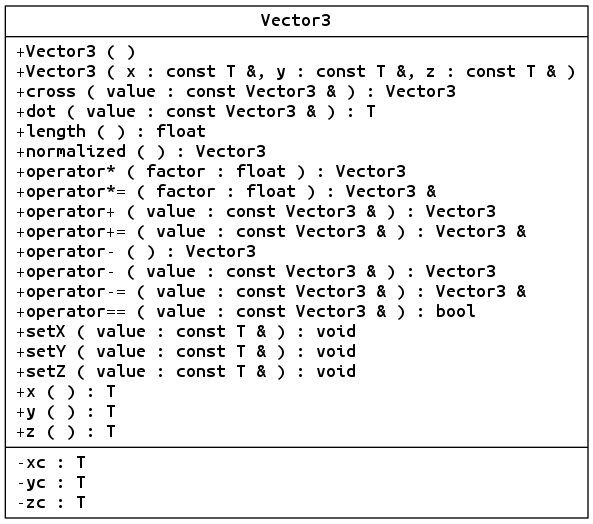
\includegraphics[scale=0.35,valign=t]{structs/Vector3.png}
%		\caption{Трехмерный вектор.}
%		\label{struct:types20}}
%\end{figure}
%\begin{figure}[H]
%	\centering
%	{
%		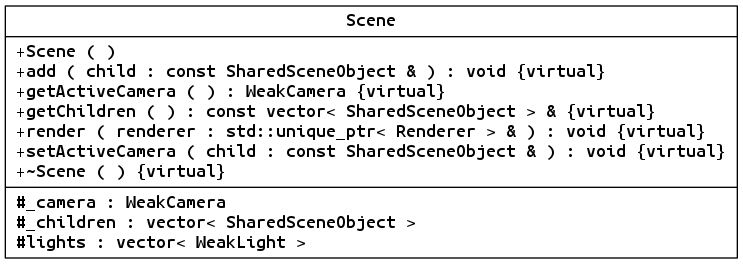
\includegraphics[scale=0.35,valign=t]{structs/Scene.png}
%		\caption{Сцена - хранит в себе все объекты, которые можно расположить на сцене: камера, модель, свет}
%		\label{struct:types22}}
%\end{figure}
%\begin{figure}[H]
%	\centering
%	{
%		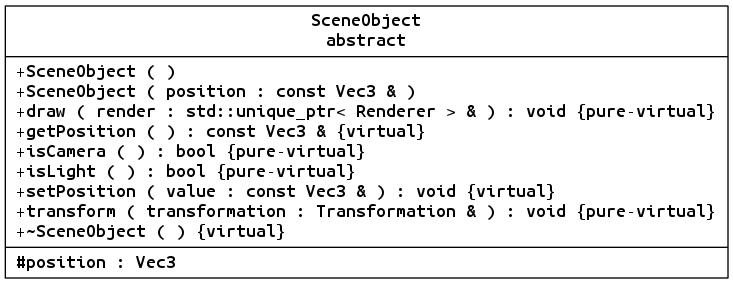
\includegraphics[scale=0.35,valign=t]{structs/SceneObject.png}
%		\caption{Абстрактный класс объекта сцены.}
%		\label{struct:types23}}
%\end{figure}
%\begin{figure}[H]
%	\centering
%	{
%		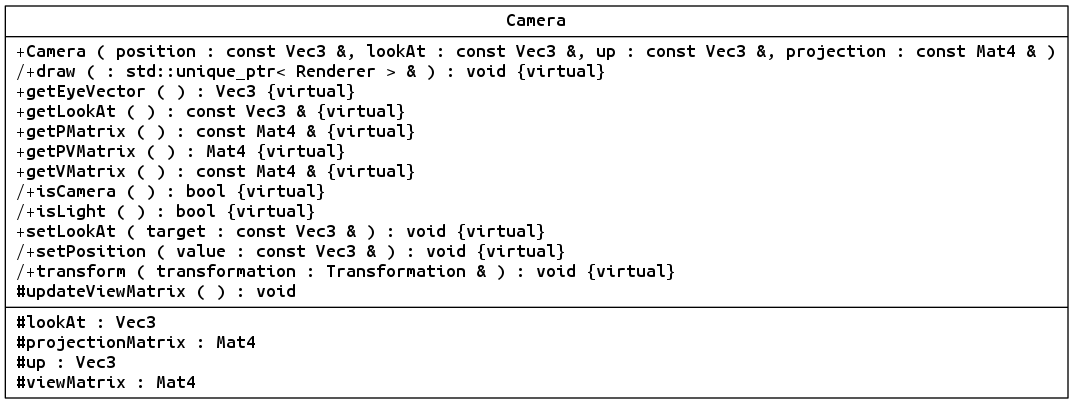
\includegraphics[scale=0.35,valign=t]{structs/Camera.png}
%		\caption{Абстрактный класс камеры.}
%		\label{struct:types24}}
%\end{figure}
%\begin{figure}[H]
%	\centering
%	{
%		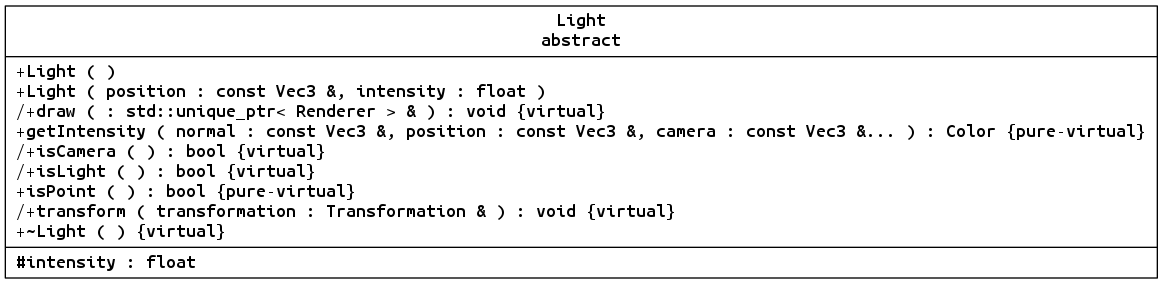
\includegraphics[scale=0.35,valign=t]{structs/Light.png}
%		\caption{Абстрактный класс света.}
%		\label{struct:types25}}
%\end{figure}
%\begin{figure}[H]
%	\centering
%	{
%		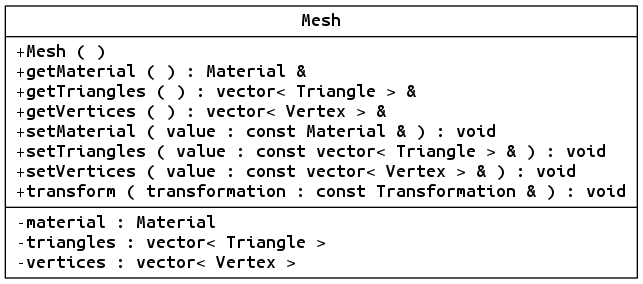
\includegraphics[scale=0.35,valign=t]{structs/Mesh.png}
%		\caption{Меш  — набор вершин и многоугольников, определяющих форму трёхмерного объекта.}
%		\label{struct:types26}}
%\end{figure}
%\begin{figure}[H]
%	\centering
%	{
%		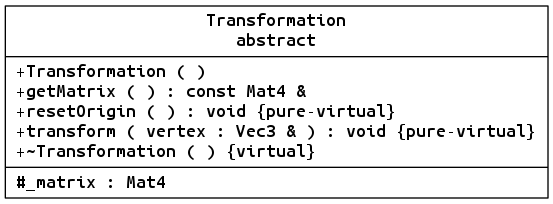
\includegraphics[scale=0.35,valign=t]{structs/Transformation.png}
%		\caption{Абстрактный класс преобразования объекта сцены.}
%		\label{struct:types27}}
%\end{figure}
%\begin{figure}[H]
%	\centering
%	{
%		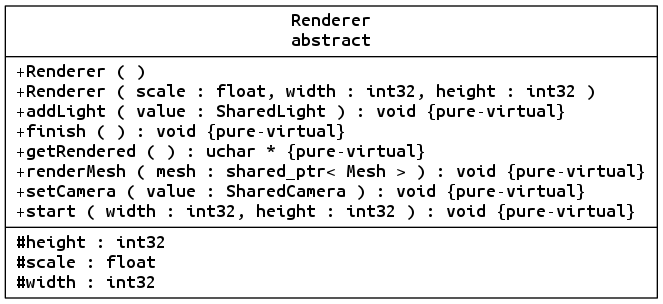
\includegraphics[scale=0.35,valign=t]{structs/Renderer.png}
%		\caption{Абстрактный класс рендера.}
%		\label{struct:types28}}
%\end{figure}


\section{Алгоритм рендеринга сцены}
Схема алгоритма рендеринга сцены представлена на рисунке \ref{fc:2}.
\begin{figure}[ht!]
	\centering{ 
		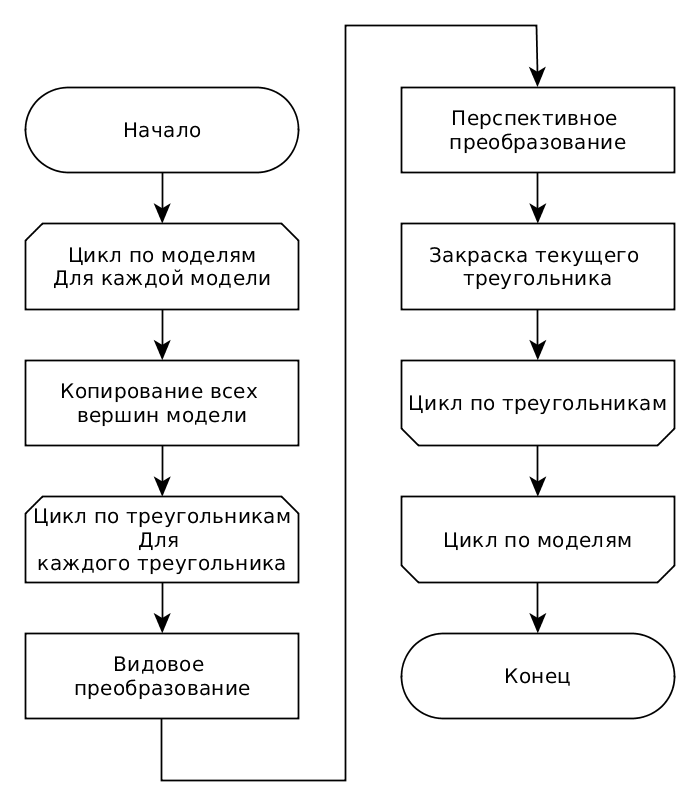
\includegraphics[width=0.68\textwidth]{img/fc2.png}
		\caption{Схема алгоритма рендеринга сцены.}
		\label{fc:2}}
\end{figure}
\section{Алгоритм закраски}
Схема алгоритма закраски треугольника представлена на рисунке \ref{fc:3.1}.
\begin{figure}[ht!]
	\centering{ 
		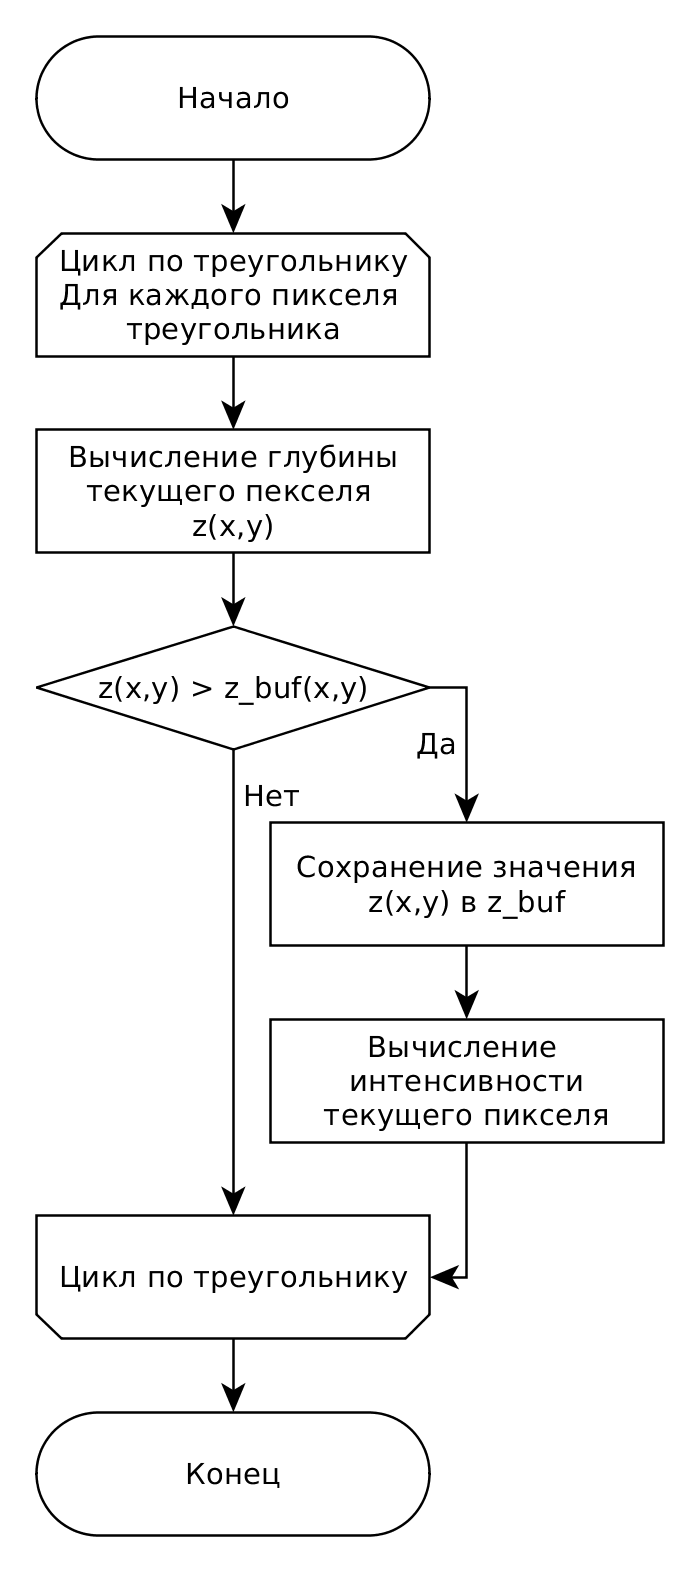
\includegraphics[width=0.5\textwidth]{img/fc3.png}
		\caption{Схема алгоритма закраски треугольника.}
		\label{fc:3.1}}
\end{figure}


\chapter{Технологический раздел}
Цель технологического раздела – описание инструментов, средств разработки, языков программирования и технологий, использованных при реализации программного комплекса системы.
\section{Выбор и обоснование языка программирования}
В качестве языка разработка был выбран C++. Причины, по которым был выбран именно он следующие:
\begin{itemize}
	\item Статическая типизация
	\item Высокая скорость выполнения
	\item Поддержка ООП
	\item Поддержка механизма исключений
	\item Последние стандарты расширили возможности языка, за счет чего разработка становится очень удобной
\end{itemize}

Выбор среды разработка пал на Qt Creator по следующим причинам:
\begin{itemize}
	\item Удобный редактор
	\item Удобные средства отладки
	\item Поддержка псевдо-асинхронной модели программирования
	\item Большое количество встроенных библиотек
	\item Частичная платформонезависимость
\end{itemize}

\section{Интерфейс пользователя}
\begin{figure}[H]
	\centering
	{
		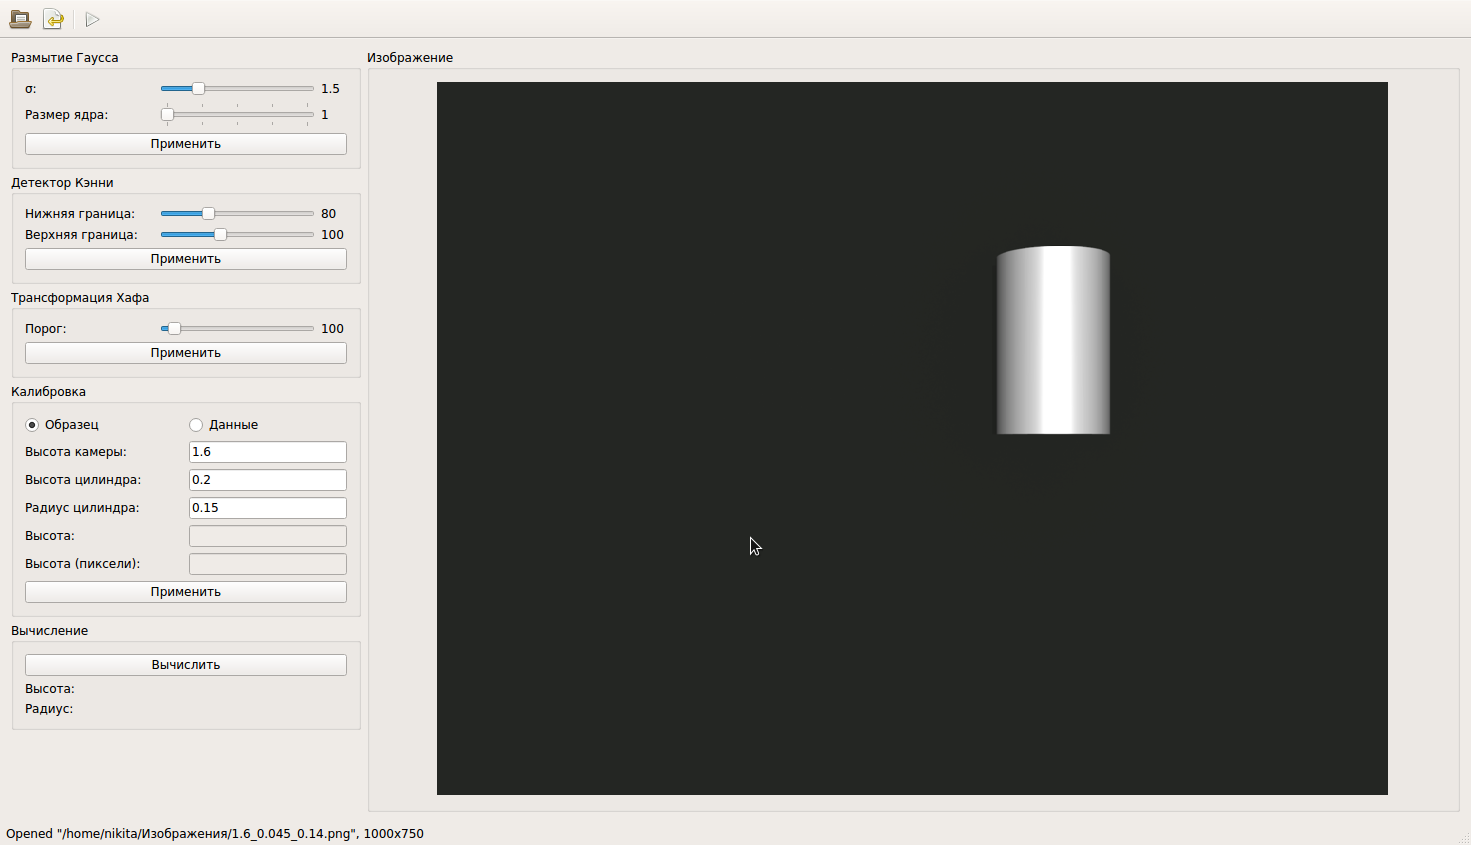
\includegraphics[scale=0.28,valign=t]{img/screen1.png}
		\caption{Главное окно.}
		\label{struct:mainwindow}}
\end{figure}
\begin{figure}[H]
	\centering
	{
		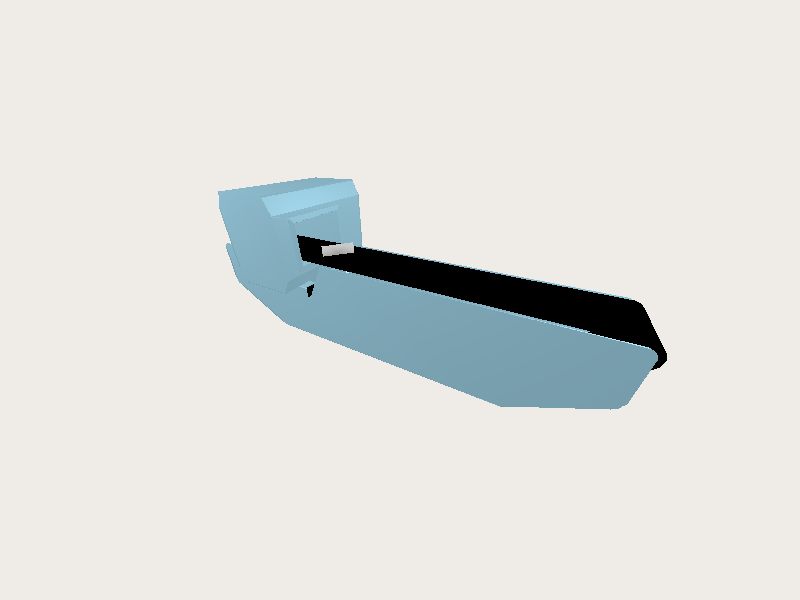
\includegraphics[scale=0.28,valign=t]{img/screen2.png}
		\caption{Окно анимации.}
		\label{struct:animation}}
\end{figure}

\section{Входные данные}
Для работы алгоритма Кэнни необходимо задать: \(\sigma \in [0..5]\) и размер ядра \(\in \overline{1,3..9}\) для сглаживания Гаусса, нижнюю и верхнюю границу пороговой фильтрации \(\in \overline{10,240}\).

Для настройки преобразования Хафа необходимо задать минимальную длину искомого отрезка \(\in \overline{10,1000}\).

Также необходимо провести калибровку системы. Сделать это можно двумя путями:
\begin{enumerate}
	\item На основе фотографии цилиндра, с известными размерами. В этом случае необходимо задать высоту камеры относительно ленты конвейера, геометрические размеры цилиндра, изображенного на фотографии.
	\item На произвольного отрезка на самой ленте конвейера. Требуется указать действительную длину этого отрезка, и длину этого отрезка на изображении в пикселях.
\end{enumerate}

\section{Основные диаграммы классов модуля нахождения размеров}
Диаграммы классов и пояснения к ним представлены на рисунках.

\begin{figure}[H]
	\centering
	\begin{minipage}{.5\textwidth}
		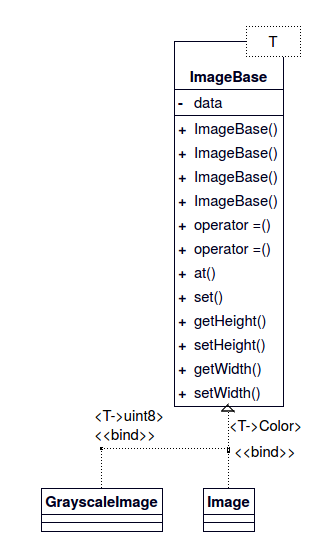
\includegraphics[scale=0.65]{classes/image.png}
		\caption{Диаграмма классов изображения.}
		\label{class:image}
	\end{minipage}%
	\begin{minipage}{.5\textwidth}
		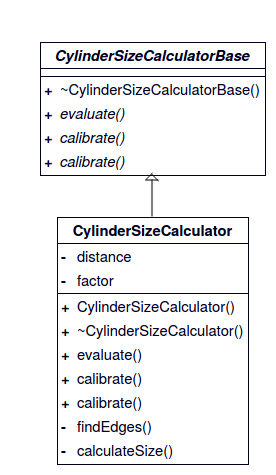
\includegraphics[scale=0.65]{classes/cylindersize.png}
		\caption{Диаграмма классов вычислительного модуля. Использован паттерн стратегия, для возможности безболезненной замены.}
		\label{class:cylindersize}
	\end{minipage}
	
\end{figure}

\begin{figure}[H]
	\centering
	\begin{minipage}{.33\textwidth}
		\centering
		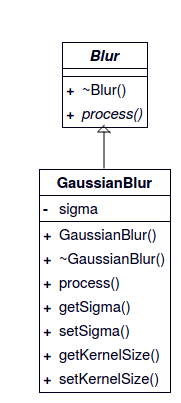
\includegraphics[scale=0.65]{classes/blur.png}
		\caption{Диаграмма классов размытия. Паттерн стратегия.}
		\label{class:blur}
	\end{minipage}%
	\begin{minipage}{.33\textwidth}
		\centering
		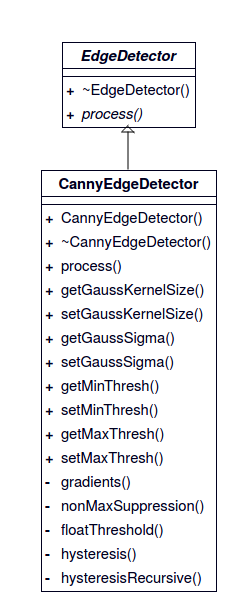
\includegraphics[scale=0.65]{classes/edgedetector.png}
		\caption{Диаграмма классов детектора границ. Паттерн стратегия.}
		\label{class:edgedetector}
	\end{minipage}
	\begin{minipage}{.33\textwidth}
		\centering
		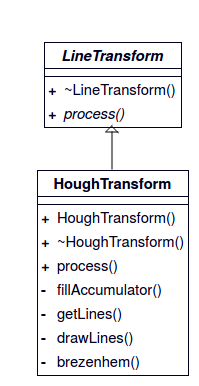
\includegraphics[scale=0.65]{classes/linetransform.png}
		\caption{Диаграмма классов детектора прямой. Паттерн стратегия.}
		\label{class:linetransform}
	\end{minipage}
\end{figure}

\section{Основные диаграммы классов модуля моделирования}
Диаграммы классов и пояснения к ним представлены на рисунках.
\begin{figure}[H]
	\centering
	\begin{minipage}{1\textwidth}
		\centering
		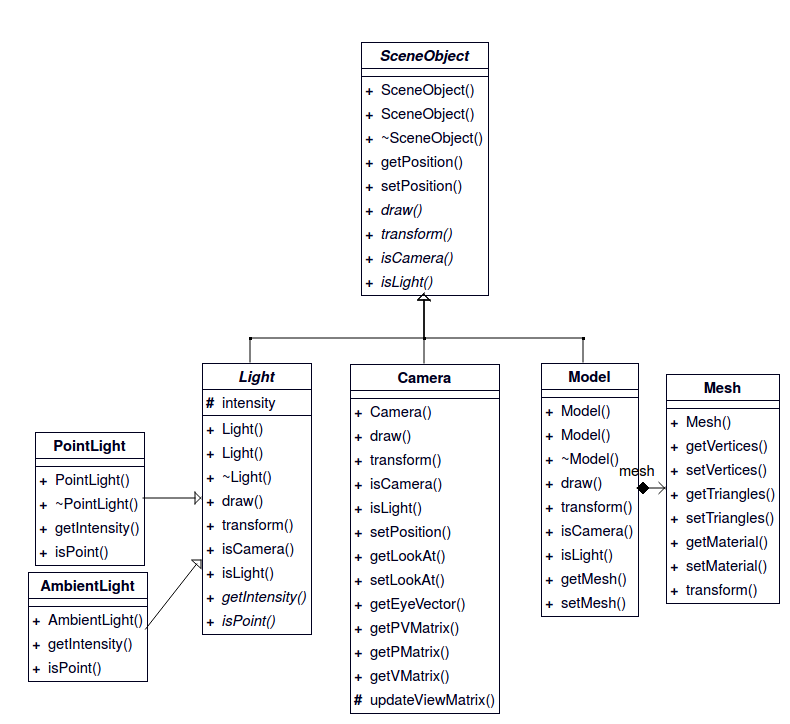
\includegraphics[scale=0.65]{classes/sceneobject.png}
		\caption{Диаграмма класс объектов сцены.}
		\label{class:sceneobject}
	\end{minipage}%
\end{figure}

\begin{figure}[H]
	\centering
	\begin{minipage}{1\textwidth}
		\centering
		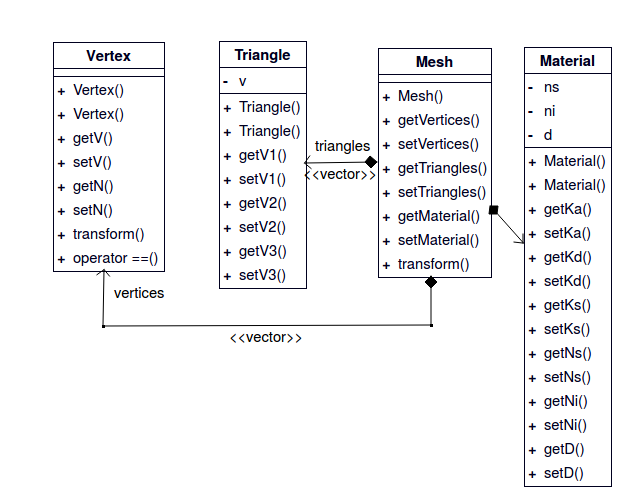
\includegraphics[scale=0.65]{classes/mesh.png}
		\caption{Диаграмма класс объектов меша.}
		\label{class:mesh}
	\end{minipage}%
\end{figure}

\begin{figure}[H]
	\centering
	\begin{minipage}{1\textwidth}
		\centering
		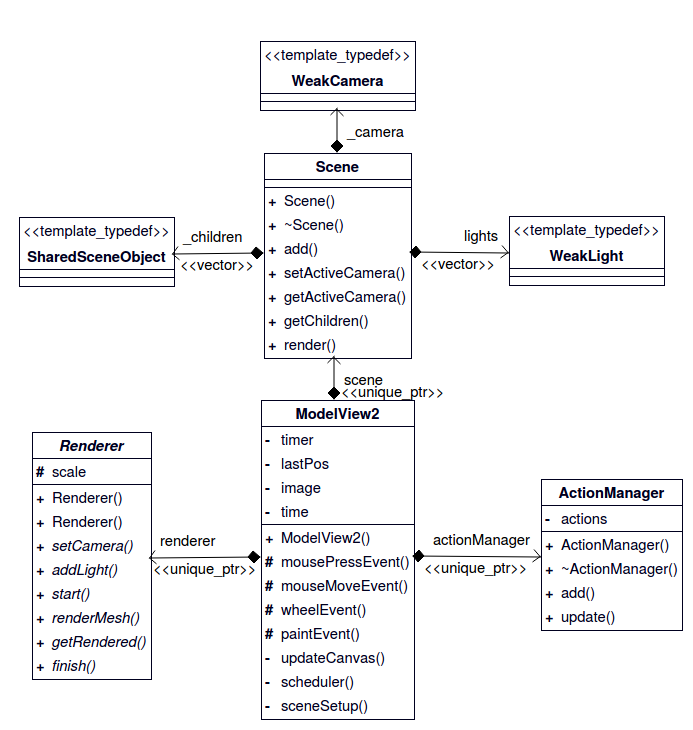
\includegraphics[scale=0.65]{classes/scene.png}
		\caption{Диаграмма классов сцены, рендера и менеджера анимаций. Для рендера использован паттерн посетитель, для абстрагирования от конкретных операций отрисовки для каждого объекта. }
		\label{class:scene}
	\end{minipage}%
\end{figure}

\begin{figure}[H]
	\centering
	\begin{minipage}{1\textwidth}
		\centering
		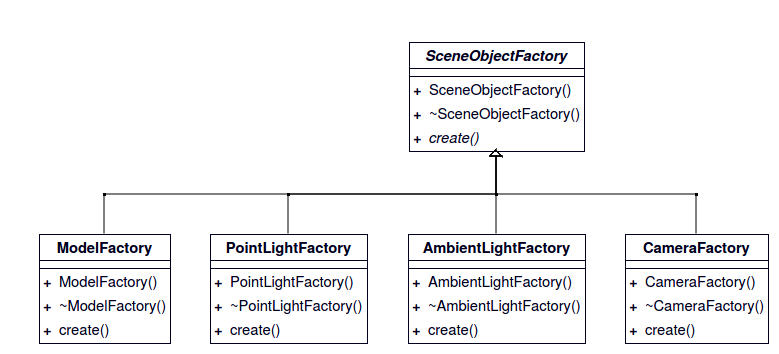
\includegraphics[scale=0.65]{classes/factory.png}
		\caption{Фабрика объектов. Паттерн фабричный метод.}
		\label{class:factory}
	\end{minipage}%
\end{figure}

\begin{figure}[H]
	\begin{minipage}{1\textwidth}
		\centering
		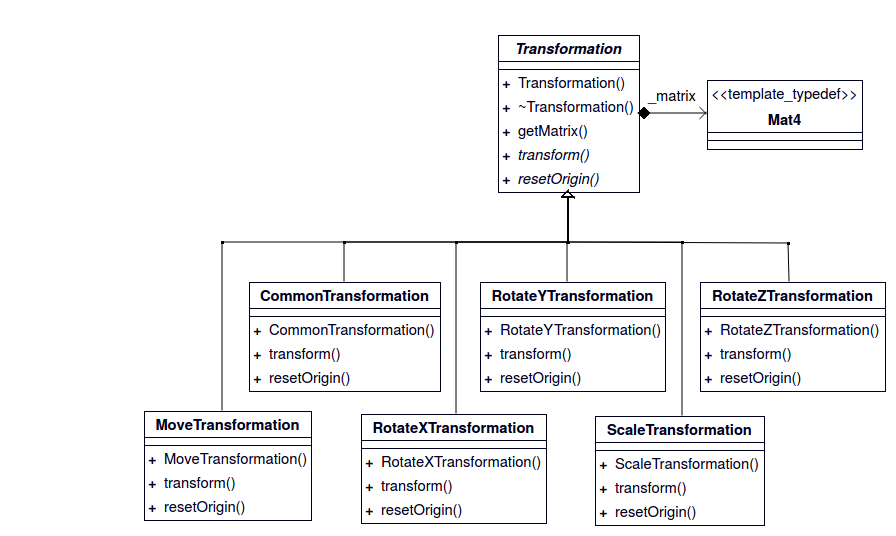
\includegraphics[scale=0.65]{classes/transformation.png}
		\caption{Диаграмма классов трансформации объектов сцены. Паттерн стратегия.}
		\label{class:transformation}
	\end{minipage}%
\end{figure}
\chapter{Экспериментальный раздел}
Цель экспериментального раздела – пример работы программы, расчет погрешности.

\section{Погрешность измерения размером цилиндра}
Для тестирования было взято три различных цилиндра, сфотографированных с высоты 1 метр 60 сантиметром:
\begin{figure}[H]
	\centering
	\begin{minipage}{.5\textwidth}
		\centering
		
\includegraphics[scale=0.2]{img/16_0045_014.png}
		\caption{Цилиндр 1. Высота 14 сантиметров, радиус 4.5 сантиметра.}
		\label{class:c1}
	\end{minipage}%
	\begin{minipage}{.5\textwidth}
		\centering
		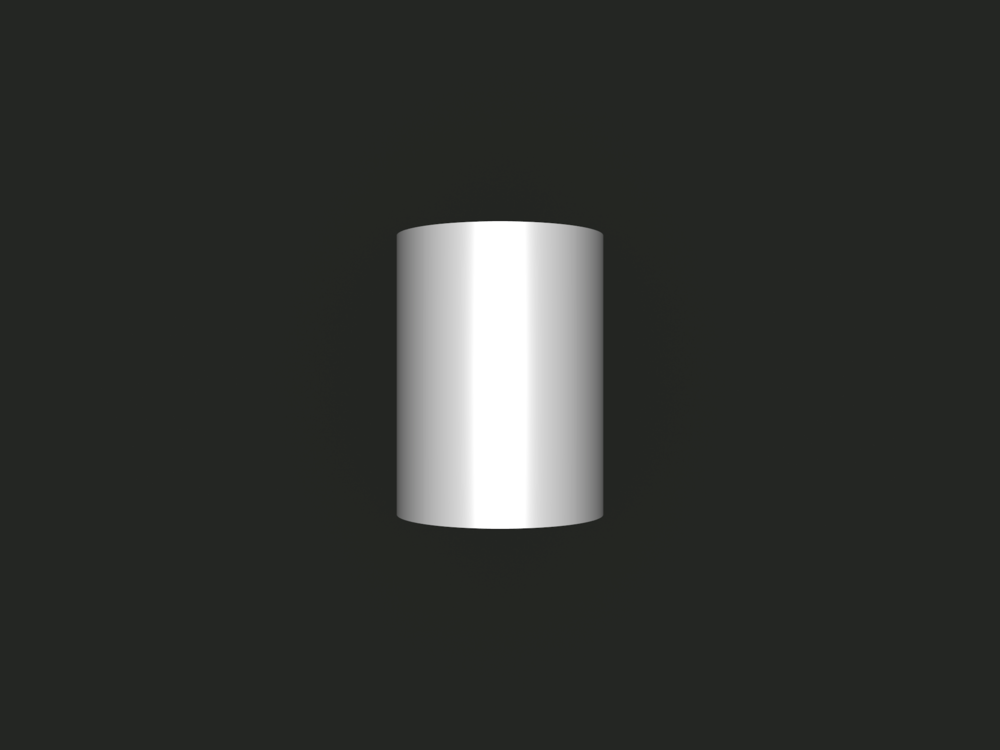
\includegraphics[scale=0.2]{img/16_0075_02.png}
		\caption{Цилиндр 2. Высота 20 сантиметров, радиус 7.5 сантиметра.}
		\label{class:c2}
	\end{minipage}
\end{figure}
\begin{figure}[H]
	\centering

	\begin{minipage}{1\textwidth}
		\centering
		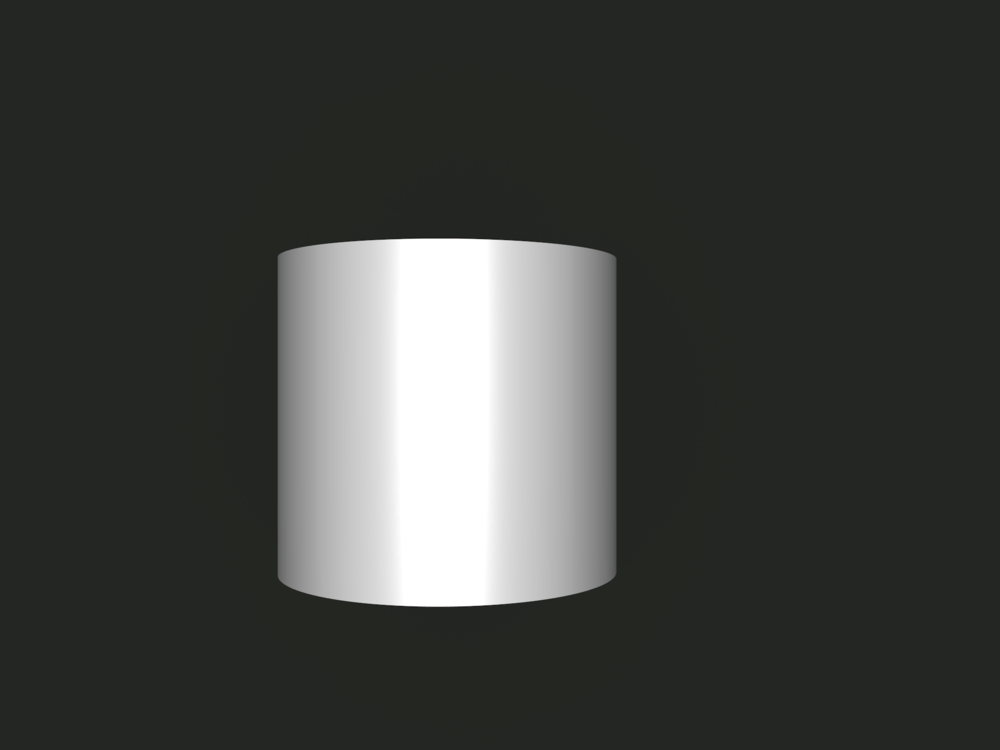
\includegraphics[scale=0.2]{img/16_0115_021.png}
		\caption{Цилиндр 3. Высота 21 сантиметр, радиус 11.5 сантиметра.}
		\label{class:c3}
	\end{minipage}
\end{figure}

В таблице \ref{tbl:1} приведены результаты тестирования:
\begin{table}[H]
	\centering
	\begin{tabular}{|l|l|l|l|l|l|}
		\hline
		\multicolumn{2}{|l|}{\backslashbox{Измерение}{Калибровка}}                                                                    & Цилиндр 1                                                         & Цилиндр 2                                                         & Цилиндр 3                                                         & Отрезок                                                 \\ \hline
		Цилиндр 1 & \begin{tabular}[c]{@{}l@{}}Радиус, м\\ Погрешность, \%\\ Высота, м\\ Погрешность, \%\end{tabular} & \begin{tabular}[c]{@{}l@{}}0.044\\ 1.2\\ 0.14\\ 0\end{tabular}    & \begin{tabular}[c]{@{}l@{}}0.043\\ 4.4\\ 0.136\\ 2.8\end{tabular} & \begin{tabular}[c]{@{}l@{}}0.041\\ 8.8\\ 0.129\\ 8.5\end{tabular} & \begin{tabular}[c]{@{}l@{}}0.046\\ 2.2\\ 0.144\\ 2.8\end{tabular} \\ \hline
		Цилиндр 2 & \begin{tabular}[c]{@{}l@{}}Радиус, м\\ Погрешность, \%\\ Высота, м\\ Погрешность, \%\end{tabular} & \begin{tabular}[c]{@{}l@{}}0.076\\ 1.3\\ 0.205\\ 2.5\end{tabular} & \begin{tabular}[c]{@{}l@{}}0.074\\ 1.3\\ 0.2\\ 0\end{tabular}     & \begin{tabular}[c]{@{}l@{}}0.071\\ 5.3\\ 0.189\\ 5.5\end{tabular} & \begin{tabular}[c]{@{}l@{}}0.78\\ 4.4\\ 0.211\\ 4.4\end{tabular}  \\ \hline
		Цилиндр 3 & \begin{tabular}[c]{@{}l@{}}Радиус, м\\ Погрешность, \%\\ Высота, м\\ Погрешность, \%\end{tabular} & \begin{tabular}[c]{@{}l@{}}0.121\\ 10\\ 0.227\\ 8.2\end{tabular}  & \begin{tabular}[c]{@{}l@{}}0.117\\ 8.3\\ 0.222\\ 5.7\end{tabular} & \begin{tabular}[c]{@{}l@{}}0.112\\ 1.8\\ 0.21\\ 0\end{tabular}    & \begin{tabular}[c]{@{}l@{}}0.124\\ 11.1\\ 0.234\\ 11\end{tabular} \\ \hline
	\end{tabular}
	\caption{Таблица погрешностей}
	\label{tbl:1}
\end{table}

Погрешность можно уменьшить, путем увеличения разрешения изображения, использованием качественных линз, которые дает наименьшую дисторсию, увеличением расстояния между камерой и объектом, чтобы была видна наибольшая часть цилиндра.
\textsl{}

\backmatter %% Здесь заканчивается нумерованная часть документа и начинаются ссылки и

\include{5-outro}
            %% заключение

%\include{60-conclusion}

%\include{61-biblio}

%\appendix   % Тут идут приложения

%\include{90-appendix1}
%\include{91-appendix2}

\end{document}

%%% Local Variables:
%%% mode: latex
%%% TeX-master: t
%%% End:
